\documentclass[12pt,a4paper]{article}
\usepackage{amsmath}
\usepackage{amsfonts}
\usepackage{amssymb}
\usepackage{graphicx}
\usepackage{secdot}
\usepackage[left=2cm,right=2cm,top=2cm,bottom=2cm]{geometry}

\author{ Shibayan Biswas, AE21B109\\ Department of Aerospace Engineering\\ IIT Madras}

\title{Homework- 4}

\date{September 21, 2022}

\begin{document}
\maketitle
\hline
\section{Recursive Powers:}
This program calculates the power of a number using recursion where base and exponent is entered by the user. In the above program, the function is a recursive function. If the power is zero, then the function returns 1 because any number raised to power 0 is 1. If the power is not 0, then the function recursively calls itself. The program for performing the above task along with one sample result for a random user input is shown below:
\begin{figure}[!ht]
	\begin{center}
		\framebox{
			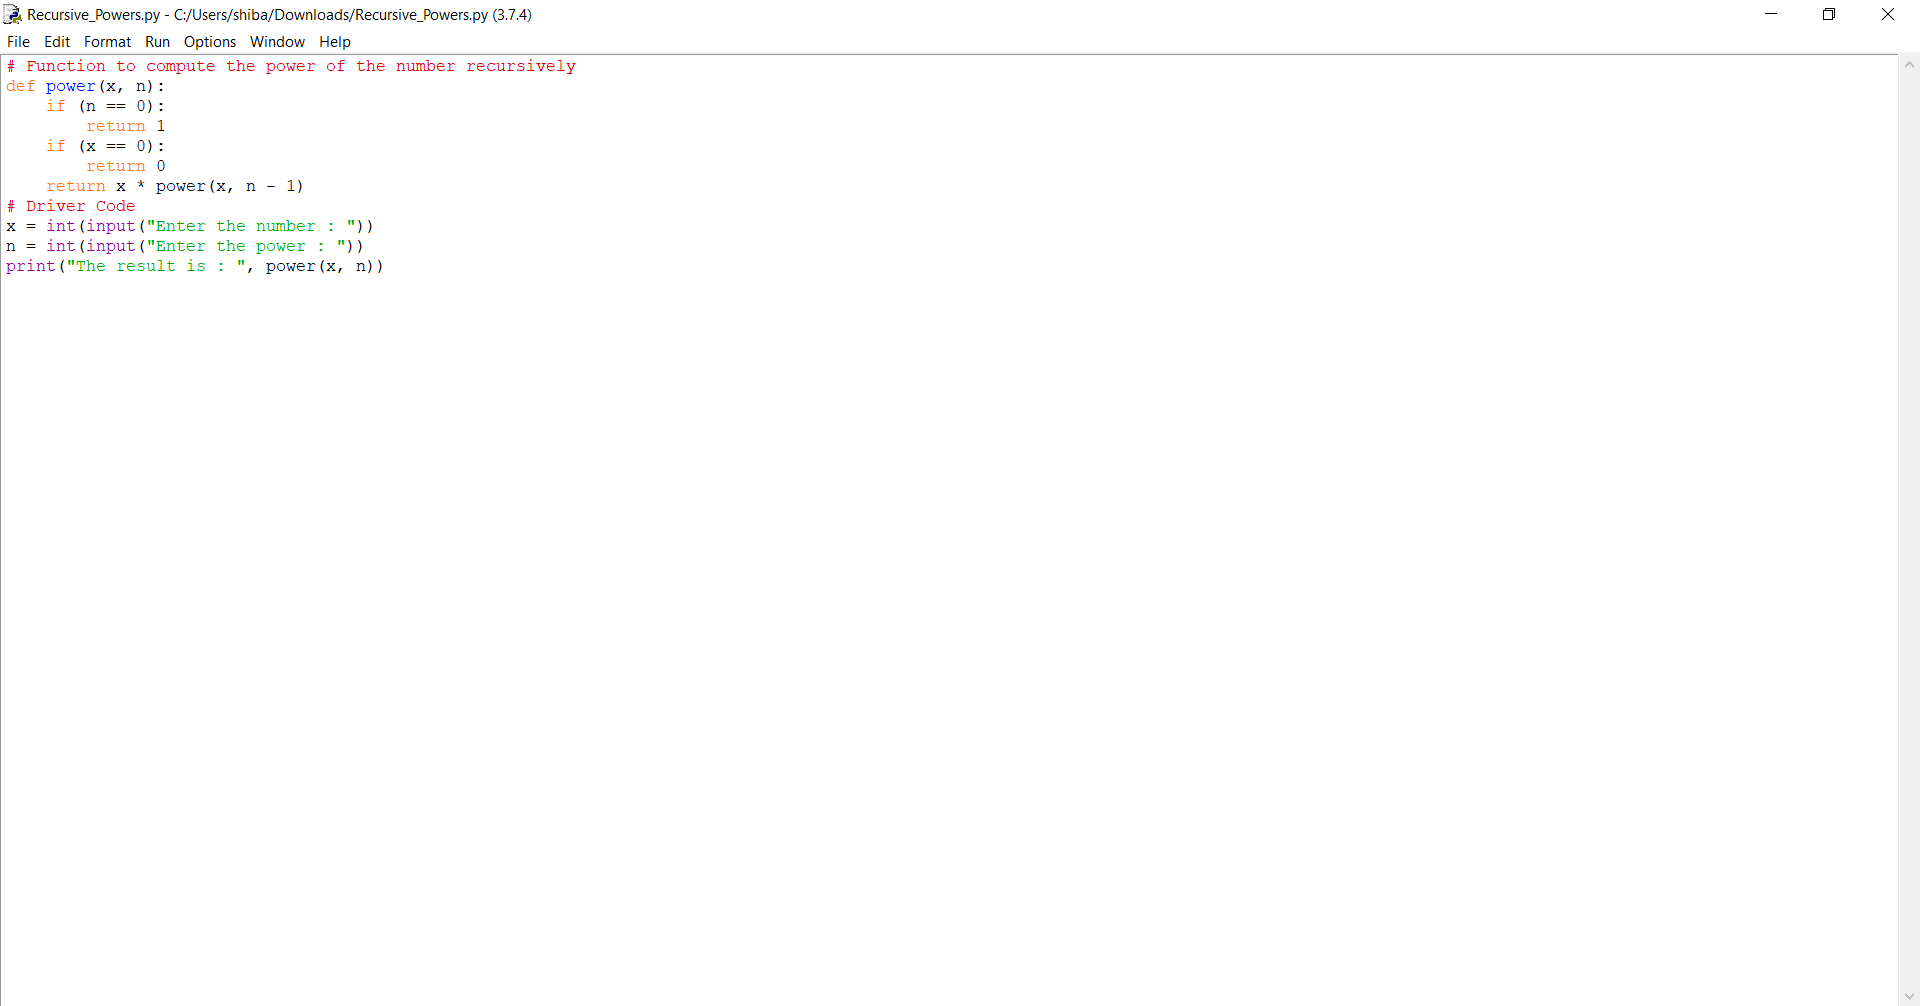
\includegraphics[scale=0.3]{Figure_1.png}
		}
	\end{center}
	\caption{Program for finding the Power of a Number recursively}
\end{figure}
\clearpage
\begin{figure}[!ht]
	\begin{center}
		\framebox{
			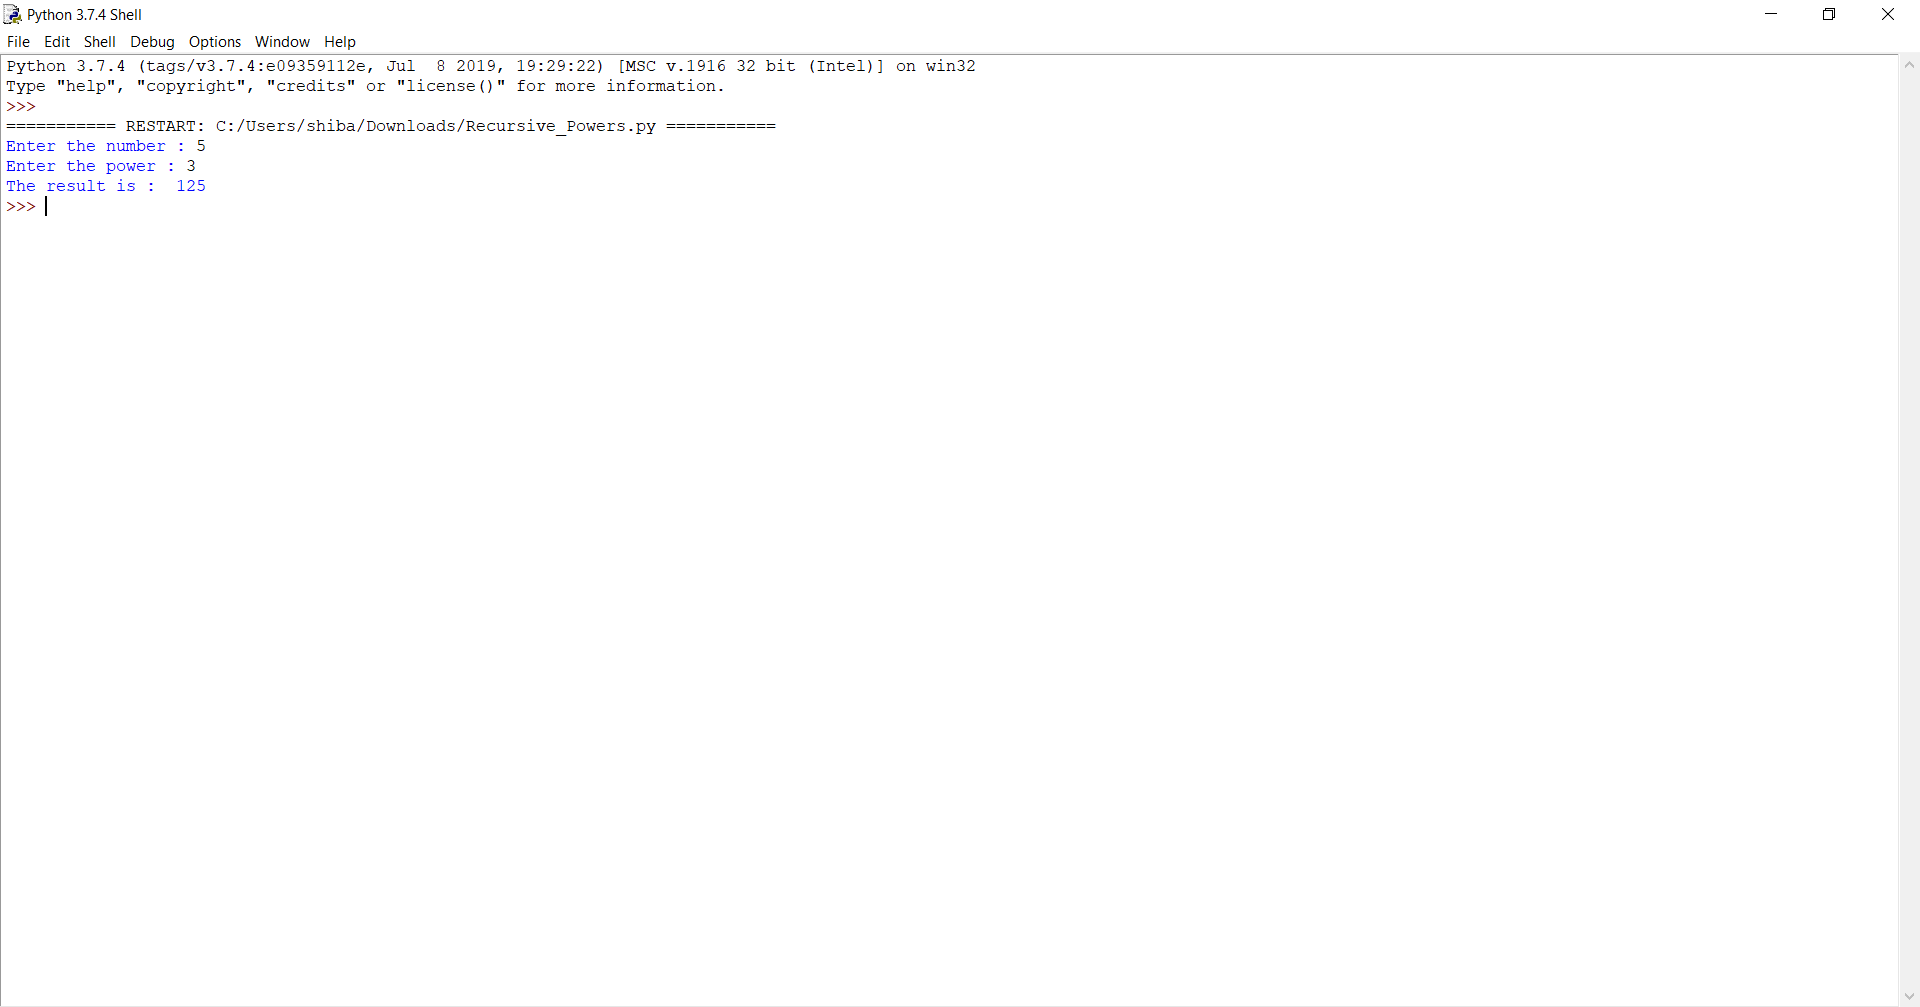
\includegraphics[scale=0.3]{Figure_2.png}
		}
	\end{center}
	\caption{Sample Output for a Random User Input}
\end{figure}
\section{The Eight Queens:}
The eight queens puzzle, or the eight queens problem, asks how to place eight queens on a chessboard without attacking each other. If you never played chess before, a queen can move in any direction (horizontally, vertically and diagonally) any number of places. In the next figure, you can see two queens with their attack patterns:
\begin{figure}[!h]
	\begin{center}
		\framebox{
			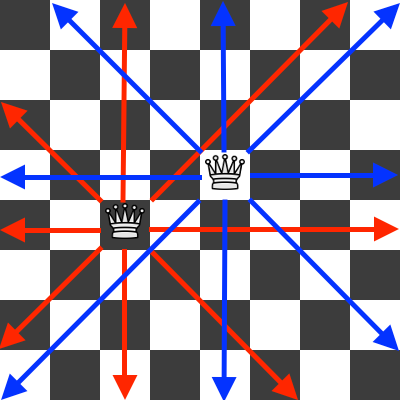
\includegraphics[scale=0.68]{Figure_3.png}
		}
	\end{center}
	\caption{Attack Patterns of Two Queens}
\end{figure}\\
We can generate a solution to the problem by scanning each row of the board and placing one queen per column, while checking at every step, that no two queens are in the line of attack of the other. A brute force approach to the problem will be to generate all possible combinations of the eight queens on the chessboard and reject the invalid states. How many combinations of 8 queens on a 64 cells chessboard are possible ? The combinations formula is:
\begin{equation}
\text{C}(n, k) = \frac{\text{n!}}{\text{k! (n - k)!}}
\end{equation}
which, for our particular case is:
\begin{equation}
\text{C}(64, 8) = 4,426,165,368
\end{equation}
Clearly, the brute force approach is not practical!\\
\\We can further reduce the number of potential solutions if we observe that a valid solution can have only one queen per row, which means that we can represent the board as an array of eight elements, where each entry represents the column position of the queen from a particular row. Take as an example the next solution of the problem:
\begin{figure}[!h]
	\begin{center}
		\framebox{
			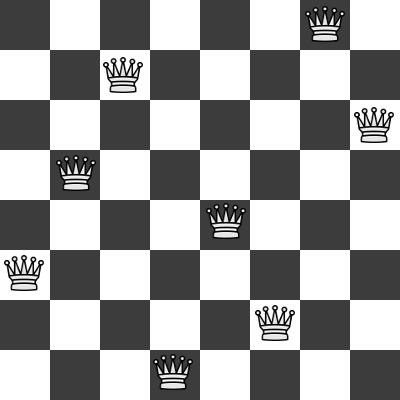
\includegraphics[scale=0.68]{Figure_4.png}
		}
	\end{center}
\end{figure}\\
The queens positions on the above board, can be represented as the occupied positions of a two dimensional 8 x 8 array: [0, 6], [1, 2], [2, 7], [3, 1], [4, 4], [5, 0], [6, 5], [7, 3]. Or, as described above, we can use a one dimensional 8 elements array: [6, 2, 7, 1, 4, 0, 5, 3].\\
\\If we look closely at the example solution [6, 2, 7, 1, 4, 0, 5, 3], we note that a potential solution to the eight queens puzzle can be constructed by generating all possible permutations of an array of eight numbers, [0, 1, 2, 3, 4, 5, 6, 7], and rejecting the invalid states (the ones in which any two queens can attack each other). The number of all permutations of n unique objects is n!, which for our particular case is 40,320 which is more reasonable than the previous 4,426,165,368 situations to analyze for the brute force approach.\\
\subsection{A more efficient solution to the puzzle uses a recursive approach:}
Assume that we’ve already generated all possible ways to place k queens on the first k rows. In order to generate the valid positions for the (k + 1) queen we place a queen on all columns of row (k + 1) and we reject the invalid states. We do the above steps until all eight queens are placed on the board. This approach will generate all 92 distinct solutions for the eight queens puzzle.
\section{The Towers of Hanoi:}
Tower of Hanoi is a mathematical puzzle where we have three rods (A, B, and C) and N disks. Initially, all the disks are stacked in decreasing value of diameter i.e., the smallest disk is placed on the top and they are on rod A. The objective of the puzzle is to move the entire stack to another rod (here considered C), obeying the following simple rules:
\begin{itemize}
\item Only one disk can be moved at a time.
\item Each move consists of taking the upper disk from one of the stacks and placing it on top of another stack; a disk can only be moved if it is the uppermost disk on a stack.
\item No disk may be placed on top of a smaller disk.
\end{itemize}
\begin{figure}[!h]
	\begin{center}
			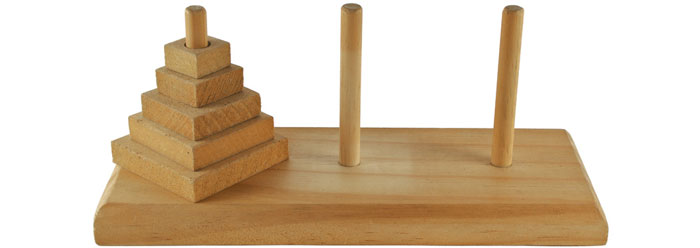
\includegraphics[scale=0.8]{Figure_6.jpg}
	\end{center}
	\caption{Setup for "The Tower of Hanoi" puzzle }
\end{figure}
\subsection{Design and Analysis of the Algorithm used:}
The idea used to solve this particular problem is to use the helper node to reach the destination using recursion. Below is the pattern for this problem:
\begin{itemize}
\item Shift ‘(N - 1)’ disks from ‘A’ to ‘B’, using C.
\item Shift last disk from ‘A’ to ‘C’.
\item Shift ‘(N - 1)’ disks from ‘B’ to ‘C’, using A.
\end{itemize}
In the algorithm that I have used for solving this particular problem, I have followed the following steps given below:
\begin{itemize}
\item Create a function "Tower Of Hanoi" where pass the N (current number of disk), Starting Rod, Destination Rod, Auxiliary Rod.
\item Make a function call for $(N – 1)^{th}$ disk.
\item Then print the current the disk along with the Starting Rod and the Destination Rod.
\item Again make a function call for $(N – 1)^{th}$ disk.
\end{itemize}
\subsection{Plot of Minimal Number of Moves v/s Number of Initial Disks:}
The plot of of Minimal Number of Moves v/s Number of Initial Disks is represented below for a random value of disks (N = 5) taken as input from the user while testing the program:
\begin{figure}[!h]
	\begin{center}
	    \framebox{
			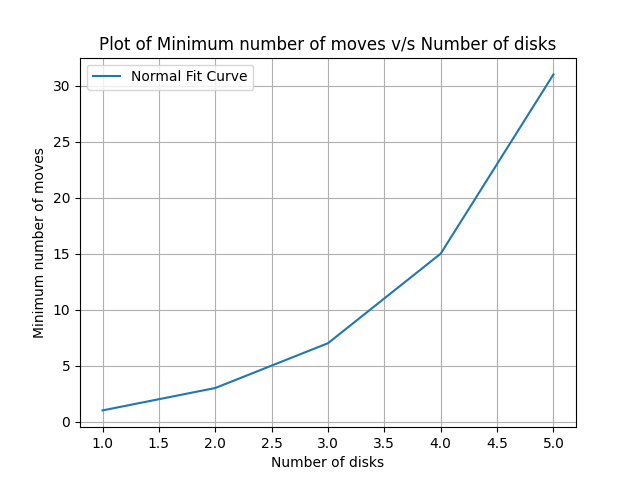
\includegraphics[scale=0.9]{Figure_5.png}
		}
	\end{center}
	\caption{Plot of Minimal Number of Moves v/s Number of Initial Disks}
\end{figure}
\subsection{Conclusions:}
\begin{itemize}
\item The most optimal solution to this problem is that we use a minimum of three pegs to interchange the positions of the disks and finally solve the problem. We will not need more than three pegs for solving this particular problem.
\item The problem cannot be solved with two pegs if the number of disks is greater than one because we will need an extra auxiliary peg for putting the disks in the correct order. 
\end{itemize}
\end{document}